% =================================================================================================
% set document class
% =================================================================================================
\documentclass[slidecentered,compress,dvipsnames,table,xcdraw,aspectratio=169]{beamer}

% =================================================================================================
% packages
% =================================================================================================
\usepackage{animate}
\usepackage{multicol}
\usepackage{algorithm}
\usepackage{algpseudocode}
\usepackage{amsmath}
\usepackage{amssymb}
\usepackage{amsthm}
\usepackage{mathtools}
\usepackage[utf8]{inputenc}
\usepackage[english]{babel}
% \usepackage[T1]{fontenc}		% not removing this so that you rememeber; adding this makes fonts jaggedy
\usepackage{tcolorbox}
% \RequirePackage{fix-cm}		% also, this one makes the fonts thinner (not strokes; the actual size)
\usepackage{transparent}
\usepackage{textpos}
\usepackage{tikz}
\usepackage{xstring}	% need for soul \hl
\usefonttheme{professionalfonts}
\usefonttheme[onlymath]{serif}
\usepackage{contour}
\usepackage{ulem}
\usepackage{soul}
\usepackage{svg}
\usepackage{calligra}
%\usepackage[style=ieee]{biblatex}
\usepackage[pro]{fontawesome5}
\usepackage{graphicx}
\usepackage{lipsum}
\usepackage{xcolor}
\usepackage[style=verbose]{biblatex}
\usepackage{pgfplots}
\usepackage{amsfonts}
\usepackage{array}
\usepackage{bm}
\usepackage{breakcites}
\usepackage{color}
\usepackage{comment}
\usepackage{float}
\usepackage{gensymb}
\usepackage{multirow}
\usepackage{pdfpages}
\usepackage[caption=false,font=footnotesize,subrefformat=parens,labelformat=parens]{subfig}
\usepackage{textcomp}
\usepackage{wrapfig}
\usepackage{tabularx}

% =================================================================================================
% settings for customization
% =================================================================================================

% set the inkscape .exe path here. needed to include svg directly
\setsvg{inkscape = "C:/Program Files/Inkscape/inkscape.exe" -z -D}

% tikz libraries
\usetikzlibrary{shadows}

% Numbered captions of tables, pictures, etc.
\setbeamertemplate{caption}[numbered]

% Bibliography settings
\addbibresource{references.bib}
\setbeamertemplate{bibliography item}{\insertbiblabel}

% set graphics path
\graphicspath{{figures/}}

% get rid of tiny navigation buttons; never use it anyway
\beamertemplatenavigationsymbolsempty

% set the footnote size to tiny
\setbeamerfont{footnote}{size=\tiny}
% add extra space to accomodate progress bar
\setbeamertemplate{footline}{\vspace{7pt}}
% adjust footnote separation to save space
\setlength{\footnotesep}{0.18cm}

% set footnote color
\setbeamercolor{footnote}{fg=STEEL_BLUE_2}

% edit footnote footcite pattern
\makeatletter
\newbibmacro*{hypercite}{%
    \renewcommand{\@makefntext}[1]{\noindent\tiny##1}%
    \footnotetext{%
        \blxmkbibnote{foot}{%
            \printtext[labelnumberwidth]{%
                \printfield{prefixnumber}%
                \printfield{labelnumber}%
            }%
            \addspace%
            \printnames[][1-1]{author}
            \setunit{\addcomma\addspace}
            \printfield{year}
            \setunit{\addcomma\addspace}
            \printfield{title}
        }%
    }%
}%
\DeclareCiteCommand{\hypercite}%
{\usebibmacro{cite:init}}
{\usebibmacro{hypercite}}
{}
{\usebibmacro{cite:dump}}
%
%% Redefine the \footcite command to use the reference number
%\renewcommand{\footcite}[1]{\cite{#1}\hypercite{#1}}
%\makeatother


% set bibliography font size
\renewcommand*{\bibfont}{\scriptsize}

% declare label name to compile named frames only
% \includeonlyframes{current}

% =================================================================================================
% input (import) modules
% =================================================================================================
%% math defs.tex
\newcommand{\ones}{\mathbf 1}
\newcommand{\reals}{{\mbox{\bf R}}}
\newcommand{\integers}{{\mbox{\bf Z}}}
\newcommand{\symm}{{\mbox{\bf S}}}  % symmetric matrices

\newcommand{\nullspace}{{\mathcal N}}
\newcommand{\range}{{\mathcal R}}
\newcommand{\Rank}{\mathop{\bf Rank}}
\newcommand{\Tr}{\mathop{\bf Tr}}
\newcommand{\diag}{\mathop{\bf diag}}
\newcommand{\card}{\mathop{\bf card}}
\newcommand{\rank}{\mathop{\bf rank}}
\newcommand{\conv}{\mathop{\bf conv}}
\newcommand{\prox}{\mathbf{prox}}

\newcommand{\Expect}{\mathop{\bf E{}}}
\newcommand{\Prob}{\mathop{\bf Prob}}
\newcommand{\Co}{{\mathop {\bf Co}}} % convex hull
\newcommand{\dist}{\mathop{\bf dist{}}}
\newcommand{\argmin}{\mathop{\rm argmin}}
\newcommand{\argmax}{\mathop{\rm argmax}}
\newcommand{\epi}{\mathop{\bf epi}} % epigraph
\newcommand{\Vol}{\mathop{\bf vol}}
\newcommand{\dom}{\mathop{\bf dom}} % domain
\newcommand{\intr}{\mathop{\bf int}}
\newcommand{\sign}{\mathop{\bf sign}}

\newcommand{\cf}{{\it cf.}}
\newcommand{\eg}{{\it e.g.}}
\newcommand{\ie}{{\it i.e.}}
\newcommand{\etc}{{\it etc.}}
%% define some colors (generated for Antibes)
\definecolor{PERSIAN_BLUE}{RGB}{51,51,178}
\definecolor{PERSIAN_BLUE_COMP_MUD_BROWN}{RGB}{178,114,51}
\definecolor{PERSIAN_BLUE_MONOCHROME}{RGB}{74,74,152}
\definecolor{PERSIAN_BLUE_ANALOG_1}{RGB}{114,51,178}
\definecolor{PERSIAN_BLUE_ANALOG_2}{RGB}{51,178,178}
\definecolor{PERSIAN_BLUE_SPLIT_COMP_1}{RGB}{178,146,51}
\definecolor{PERSIAN_BLUE_SPLIT_COMP_2}{RGB}{178,83,51}
\definecolor{PERSIAN_BLUE_TRIADIC_1}{RGB}{51,178,51}
\definecolor{PERSIAN_BLUE_TRIADIC_2}{RGB}{178,51,51}
\definecolor{PERSIAN_BLUE_TETRADIC_1}{RGB}{178,114,51}
\definecolor{PERSIAN_BLUE_TETRADIC_2}{RGB}{178,178,51}
\definecolor{PERSIAN_BLUE_TETRADIC_3}{RGB}{178,51,178}
\definecolor{RAISIN_BLACK}{RGB}{42,45,52}
\definecolor{RUSSIAN_GREEN}{RGB}{92,148,110}
\definecolor{BLIZZARD_BLUE}{RGB}{160,221,230}
\definecolor{DARK_ORANGE}{RGB}{255,143,41}
\definecolor{PICOTEE_BLUE}{RGB}{38,38,134}
\definecolor{BISTRE}{RGB}{55,44,37}
\definecolor{GRAY_WEB}{RGB}{131,131,131}
\definecolor{DARK_SKY_BLUE}{RGB}{147,183,190}
\definecolor{MINT_CREAM_1}{RGB}{241,255,250}
\definecolor{MINT_CREAM_2}{RGB}{247,255,247}
\definecolor{PALE_SILVER}{RGB}{213,199,188}
\definecolor{OPAL}{RGB}{148,191,190}
\definecolor{LASER_LEMON}{RGB}{252,252,98}
\definecolor{MINDARO}{RGB}{218,255,125}
\definecolor{GRANNY_SMITH_APPLE}{RGB}{178,239,155}
\definecolor{RHYTHM}{RGB}{140,134,170}
\definecolor{SILVER}{RGB}{197,197,197}
\definecolor{SPANISH_GRAY_1}{RGB}{130,145,145}
\definecolor{SPANISH_GRAY_2}{RGB}{148,155,150}
\definecolor{BRICK_RED}{RGB}{195,60,84}
\definecolor{SKY_BLUE_CRAYOLA}{RGB}{142,227,239}
\definecolor{CELESTE}{RGB}{174,243,231}
\definecolor{HOOKERS_GREEN}{RGB}{88,125,113}
\definecolor{GREEN_PANTONE}{RGB}{77,170,87}
\definecolor{NAPLES_YELLOW}{RGB}{255,130,109}
\definecolor{AIR_SUPERIORITY_BLUE}{RGB}{108,166,193}
\definecolor{FIRE_BRICK}{RGB}{179,0,27}
\definecolor{ICE_BERG}{RGB}{126,163,204}
\definecolor{TAN}{RGB}{204,173,143}
\definecolor{MIDDLE_BLUE}{RGB}{247,255,247}
\definecolor{LAVENDER_BLUSH}{RGB}{238,229,233}
\definecolor{CINNABAR}{RGB}{214,73,51}
\definecolor{BABY_POWDER}{RGB}{247,247,242}
\definecolor{AQUA_MARINE}{RGB}{133,255,199}
\definecolor{CORAL}{RGB}{255,133,82}
\definecolor{PLATINUM}{RGB}{230,230,230}
\definecolor{BROWN}{RGB}{126,89,32}
\definecolor{FULVOUS}{RGB}{220,133,31}
\definecolor{YELLOW_ORANGE}{RGB}{255,167,55}
\definecolor{BITTER_SWEET}{RGB}{255,111,89}
\definecolor{ZOMP}{RGB}{67,170,139}
\definecolor{AMARANTH_RED}{RGB}{215,29,45}
\definecolor{SPACE_CADET}{RGB}{49,61,90}
\definecolor{CELADON_BLUE}{RGB}{66,129,164}
\definecolor{ELECTRIC_BLUE}{RGB}{142, 237, 247}
\definecolor{BABY_BLUE_EYES}{RGB}{161, 205, 241}
\definecolor{STAR_COMMAND}{RGB}{34, 116, 165}
\definecolor{DENIM_BLUE}{RGB}{57, 67, 183}
\definecolor{BLUE_JEANS}{RGB}{72, 172, 240}
\definecolor{UPSDELL_RED}{RGB}{180, 24, 37}
\definecolor{RED_MUNSELL}{RGB}{228, 58, 72}
\definecolor{BLUE_MUNSELL}{RGB}{27, 154, 170}
\definecolor{LIBERTY}{RGB}{76, 76, 157}
\definecolor{BABY_BLUE}{RGB}{108, 207, 246}
\definecolor{CAROLINA_BLUE}{RGB}{27, 152, 224}
\definecolor{MINION_YELLOW}{RGB}{242, 220, 93}
\definecolor{SANDY_BROWN}{RGB}{242, 163, 89}
\definecolor{FLAME}{RGB}{215, 78, 9}
\definecolor{BLOOD_RED}{RGB}{110, 14, 10}
\definecolor{CLARET}{RGB}{137, 4, 61}
\definecolor{EMERALD}{RGB}{68, 207, 108}
\definecolor{ILLUMINATING_EMERALD}{RGB}{50, 147, 111}
\definecolor{MAROON_X_11}{RGB}{184, 19, 101}
\definecolor{CARRIBEAN_GREEN}{RGB}{29, 211, 176}
\definecolor{RED_CRAYOLA}{RGB}{239, 45, 86}
\definecolor{EGG_SHELL}{RGB}{244, 236, 214}
\definecolor{AMAZON}{RGB}{74, 120, 86}
\definecolor{GOOGLE_G}{RGB}{60, 186, 84}
\definecolor{GOOGLE_Y}{RGB}{244, 194, 13}
\definecolor{GOOGLE_R}{RGB}{219, 50, 54}
\definecolor{GOOGLE_B}{RGB}{72, 133, 237}
\definecolor{PRINCETON_ORANGE}{RGB}{245, 128, 38}
\definecolor{YALE_BLUE}{RGB}{0, 68, 128}
\definecolor{MIKADO_YELLOW}{RGB}{255, 193, 0}
\definecolor{SELECTIVE_YELLOW}{RGB}{255, 186, 8}
\definecolor{MISTY_ROSE}{RGB}{255, 227, 220}
\definecolor{HONEY_YELLOW}{RGB}{247, 179, 43}
\definecolor{RUBY_RED}{RGB}{154, 3, 30}
\definecolor{BRONZE}{RGB}{203, 121, 58}
\definecolor{CELADON}{RGB}{172,247,193}
\definecolor{GREEN_SHEEN}{RGB}{128,194,175}
\definecolor{GREEN_SHEEN_2}{RGB}{136, 183, 181}
\definecolor{CITRINE}{RGB}{224, 202, 60}
\definecolor{MELLOW_APRICOT}{RGB}{255, 184, 111}
\definecolor{GLOSSY_GRAPE}{RGB}{171,146,191}
\definecolor{PINK_LAVENDER}{RGB}{212, 178, 216}
\definecolor{MAGIC_MINT}{RGB}{139, 232, 203}
\definecolor{MANATEE}{RGB}{141, 153, 174}
\definecolor{ALICE_BLUE}{RGB}{237, 242, 244}
\definecolor{SPANISH_BISTRE}{RGB}{111, 115, 47}
\definecolor{CAMEL}{RGB}{179, 138, 88}
\definecolor{PORTLAND_ORANGE}{RGB}{244, 96, 54}
\definecolor{PERSIAN_GREEN}{RGB}{27, 153, 139}
\definecolor{BEIGE}{RGB}{235, 235, 211}
\definecolor{CERISE}{RGB}{218, 65, 103}
\definecolor{LAVENDER_BLUE}{RGB}{183, 195, 243}
\definecolor{CYCLAMEN}{RGB}{221, 117, 150}
\definecolor{POPSTAR}{RGB}{175, 93, 99}
\definecolor{FERN_GREEN}{RGB}{91, 117, 83}
\definecolor{MIDNIGHT_BLUE}{RGB}{25, 25, 89}
\definecolor{DAVYS_GRAY}{RGB}{87, 87, 97}
\definecolor{COOL_GRAY}{RGB}{132, 143, 165}
\definecolor{BATTLESHIP_GRAY}{RGB}{133, 135, 134}
\definecolor{GREEN_BLUE}{RGB}{0, 100, 177}
\definecolor{SEAL_BROWN}{RGB}{82, 43, 24}
\definecolor{CHESTNUT}{RGB}{139, 84, 61}
\definecolor{AVOCADO}{RGB}{67, 125, 3}
\definecolor{SHEEN_GREEN}{RGB}{126, 203, 1}
\definecolor{MALACHITE}{RGB}{47, 212, 82}
\definecolor{STEEL_BLUE}{RGB}{51, 123, 178}

% generated for (UTA colors) YALE_BLUE/PRINCETON_ORANGE theme
\definecolor{PRUSSIAN_BLUE}{RGB}{0, 51, 96}
\definecolor{OXFORD_BLUE}{RGB}{0, 34, 64}
\definecolor{AUBURN}{RGB}{164, 44, 45}
\definecolor{CADMIUM_ORANGE}{RGB}{237, 140, 65}
\definecolor{CASTLETON_GREEN}{RGB}{40, 89, 67}
\definecolor{BLACK_CHOCOLATE}{RGB}{35, 35, 26}
\definecolor{BITTER_LIME}{RGB}{188, 237, 9}
\definecolor{DARK_SIENNA}{RGB}{45, 6, 5}
\definecolor{TYRIAN_PURPLE}{RGB}{76, 8, 39}
\definecolor{GOLD_FUSION}{RGB}{117, 112, 78}
\definecolor{RUBY}{RGB}{216, 17, 89}
\definecolor{QUINACRIDONE_MAGENTA}{RGB}{143, 45, 86}
\definecolor{PUCE}{RGB}{195, 125, 146}
\definecolor{DEEP_TAUPE}{RGB}{132, 98, 103}
\definecolor{MOUNTBATTEN_PINK}{RGB}{147, 116, 138}
\definecolor{RED_VIOLET_CRAYOLA}{RGB}{175, 77, 152}
\definecolor{WILD_ORCHID}{RGB}{214, 107, 160}
\definecolor{MEDIUM_SLATE_BLUE}{RGB}{125, 131, 255}
\definecolor{BLUE_JEANS}{RGB}{0, 166, 251}
\definecolor{ANTIQUE_BRONZE}{RGB}{100, 101, 54}
\definecolor{OLIVE_DRAB_7}{RGB}{72, 61, 3}
\definecolor{BRIGHT_MAROON}{RGB}{179, 57, 81}
\definecolor{BOTTLE_GREEN}{RGB}{34, 111, 84}
\definecolor{WINTER_GREEN_DREAM}{RGB}{75, 143, 140}
\definecolor{LIVER}{RGB}{101, 66, 54}
\definecolor{FOREST_GREEN_CRAYOLA}{RGB}{124, 169, 130}
\definecolor{PURPLE_MOUNTAIN_MAJESTY}{RGB}{159, 134, 192}
\definecolor{LILAC}{RGB}{190, 149, 196}
\definecolor{CERULEAN_CRAYOLA}{RGB}{0, 167, 225}
\definecolor{MEDIUM_PURPLE}{RGB}{147, 129, 255}
\definecolor{PARADISE_PINK}{RGB}{236, 64, 103}
\definecolor{KOMBU_GREEN}{RGB}{36, 49, 25}
\definecolor{OPERA_MAUVE}{RGB}{200, 132, 166}
\definecolor{TITANIUM_YELLOW}{RGB}{240, 225, 0}
\definecolor{DARK_LAVA}{RGB}{82, 70, 50}
\definecolor{SPANISH_CARMINE}{RGB}{209, 17, 73}
\definecolor{SADDLE_BROWN}{RGB}{128, 47, 0}
\definecolor{INDIGO_DYE}{RGB}{21, 65, 103}
\definecolor{SEA_GREEN}{RGB}{0, 128, 60}
\definecolor{NAVY_BLUE}{RGB}{30, 0, 128}
\definecolor{BROWN}{RGB}{128, 79, 0}
\definecolor{BARN_RED}{RGB}{128, 15, 0}
\definecolor{SPANISH_BISTRE}{RGB}{128, 111, 0}
\definecolor{BURGUNDY}{RGB}{128, 0, 34}
\definecolor{INDIGO}{RGB}{94, 0, 128}
\definecolor{MAGENTA_DYE}{RGB}{198, 15, 123}
\definecolor{MAGENTA_PROCESS}{RGB}{249, 0, 147}
\definecolor{ASPARAGUS}{RGB}{136, 171, 117}
\definecolor{MAXIMUM_GREEN}{RGB}{103, 148, 54}
\definecolor{BLUE_MUNSELL}{RGB}{45, 147, 173}
\definecolor{RIFLE_GREEN}{RGB}{78, 83, 64}
\definecolor{NICKEL}{RGB}{105, 114, 104}
\definecolor{SPANISH_VIRIDIAN}{RGB}{12, 124, 89}
\definecolor{PACIFIC_BLUE}{RGB}{42, 183, 202}
\definecolor{CHARTREUSE_TRADITIONAL}{RGB}{228, 255, 26}
\definecolor{FIERY_ROSE}{RGB}{255, 83, 118}
\definecolor{LIGHT_SEA_GREEN}{RGB}{0, 166, 166}
\definecolor{YELLOW_GREEN}{RGB}{138, 201, 38}
\definecolor{FRENCH_RASPBERRY}{RGB}{195, 49, 73}
\definecolor{RADICAL_RED}{RGB}{255, 56, 100}
\definecolor{FIREBRICK}{RGB}{179, 0, 27}
\definecolor{STEEL_TEAL}{RGB}{80, 132, 132}
\definecolor{CRIMSON_UA}{RGB}{166, 38, 57}
\definecolor{ROSE}{RGB}{255, 114, 118}
\definecolor{INDIGO_2}{RGB}{99, 93, 198}
\definecolor{HONEY_DEW}{RGB}{213, 242, 227}
\definecolor{STEEL_BLUE_2}{RGB}{89, 133, 170}
\definecolor{CAMBRIDGE_BLUE}{RGB}{167, 202, 177}
\definecolor{ORANGE_WEB}{RGB}{255, 164, 0}
\definecolor{CAROLINA_BLUE_2}{RGB}{0, 159, 253}


\definecolor{YALE_BLUE}{RGB}{0, 68, 124}


% always comment below line until last compile. It takes a while to add progress bar features on slides.
%\input{./progress_bar}

% set global color for normal text (almost black)
\setbeamercolor{normal text}{fg=BLACK_CHOCOLATE}

% =================================================================================================
% set mode and theme
% =================================================================================================
\mode<presentation>{\usetheme{Antibes}\usecolortheme[named=YALE_BLUE]{structure}}


% =================================================================================================
% new command definitions
% =================================================================================================
% \newcommand{\fnt}[1]{\fontsize{#1}{0}\selectfont}

% tikzmark can be used to draw things like arbitrary arrows between two marked points
% usage: \tikzmark{mark1}
\newcommand\tikzmark[1]{\tikz[overlay, remember picture] \node (#1) {};}

% helper command to display circle with given color and name
% usage: \colorshow{BRIGHT_MAROON}
\newcommand{\colorshow}[1]{
    \begin{tikzpicture}
        \node[fill=#1,
            circle,
            minimum size=2ex,
            label={\tiny \StrSubstitute{#1}{_}{\ }},
        ] at (0,0){};
    \end{tikzpicture}
}

% helper command to set inactive text
\newcommand{\unemph}[1]{\texttransparent{0.2}{#1}}

% renew underline \myul
% \myul will underline closer not cutting through p's and y's hanging tails
% for the usual underline use \ul
\renewcommand{\ULdepth}{1.8pt}
\contourlength{0.8pt}

\newcommand{\myul}[1]{%
    \uline{\phantom{#1}}%
    \llap{\contour{white}{#1}}%
}
\makeatletter
\let\HL\hl
\renewcommand{\hl}{%
    \let\set@color\beamerorig@set@color
    \let\reset@color\beamerorig@reset@color
    \HL}
\makeatother

% set the highlight color
% usage: \hl{dummy text}
\sethlcolor{MINDARO}


% =================================================================================================
% define title
% =================================================================================================
\title[{Variable Rate Compression for Raw 3D Point Clouds}]{
        {Variable Rate Compression for Raw 3D Point Clouds}
}

%\subtitle{\small A second date}
\author{\textcolor{RAISIN_BLACK}{Md Ahmed Al Muzaddid and William J. Beksi}\\ICRA, 2022}
\institute{
    
\includegraphics[height=1cm]{figures/uta_logo}\newline \newline
    \textcolor{BRIGHT_MAROON}{\bf \small University of Texas, Arlington} \newline
    \textcolor{NICKEL}{\tiny 05/24/2022}\newline \newline
}
% RVL logo
\titlegraphic{\vspace{-15mm}\includegraphics[height=1cm]{icra_logo_full} \hfill 
\includegraphics[height=1cm]{rvl_logo_2.pdf}}
\date{}


%%%%%%%%%%%%%%%%%%%%%%%%%%%%%%%%%%%%%%%%%%%%%%%%%%%%%%%%%%%%%%%%%%%%%%%%%%%%%%%%%%%%%%%%%%%%%%%%%%%
%%%%%%%%%%%%%%%%%%%%%%%%%%%%%%%%%%%%%%%%%%%%%%%%%%%%%%%%%%%%%%%%%%%%%%%%%%%%%%%%%%%%%%%%%%%%%%%%%%%

% =================================================================================================
% DOCUMENT BEGINS HERE
% =================================================================================================
\begin{document}

% -------------------------------------------------------------------------------------------------
% title
% -------------------------------------------------------------------------------------------------
%% title frame
    \begin{frame}
        \titlepage
    \end{frame}

% UTA logo on all frames after
    \addtobeamertemplate{frametitle}{}{
        \begin{textblock*}{100mm}(0.95\textwidth,-0.96cm)
            
\includegraphics[height=0.95cm,]{icra_logo_inverse}
        \end{textblock*}
    }

% -------------------------------------------------------------------------------------------------
% table of contents
% -------------------------------------------------------------------------------------------------
% %% ToC
% \begin{frame}{Outline}
% 	\tableofcontents
% \end{frame}

% %% ToC at beginning of sections
% \AtBeginSection[]
% {
% \begin{frame}{Outline}
% 	\tableofcontents[currentsection]
% \end{frame}
% }

% %% ToC at beginning of subsections
% \AtBeginSubsection[]
% {
% \begin{frame}{Outline}
% 	\tableofcontents[currentsubsection]
% \end{frame}
% }


%    \begin{frame}{Outline}
%        \begin{multicols}{2}
%            \tableofcontents[sections={1-8}]
%        \end{multicols}
%    \end{frame}


%% ToC at begin of sections
    \AtBeginSection[]
    {
        \begin{frame}{Outline}
            \begin{multicols}{2}
                \tableofcontents[sections={1-8}, currentsection]
            \end{multicols}
        \end{frame}
    }
%% ToC at being subsections
    \AtBeginSubsection[]
    {
        \begin{frame}{Outline}
            \begin{multicols}{2}
                \tableofcontents[sections={1-8}, currentsubsection]
            \end{multicols}
        \end{frame}
    }

%%%%%%%%%%%%%%%%%%%%%%%%%%%%%%%%%%%%%%%%%%%%%%%%%%%%%%%%%%%%%%%%%%%%%%%%%%%%%%%%%%%%%%%%%%%%%%%%%%%
% =================================================================================================
% MAIN CONTENT STARTS HERE
% =================================================================================================

% -------------------------------------------------------------------------------------------------
% introduction
% -------------------------------------------------------------------------------------------------


    \begin{frame}{Learning based 3D compression}
        \begin{columns}
            \column{0.5\textwidth}
            \only<1>{
                \begin{itemize}
                \item Inspired by learning  based Image compression
                \item Unlike 2D image, the structure of a 3D point cloud is irregular
                \item To overcome irregularity, point clouds are typically voxelized\footcite{ozbay2019voxelize}
                \end{itemize}
            }
            \column{0.5\textwidth}
            \centering
            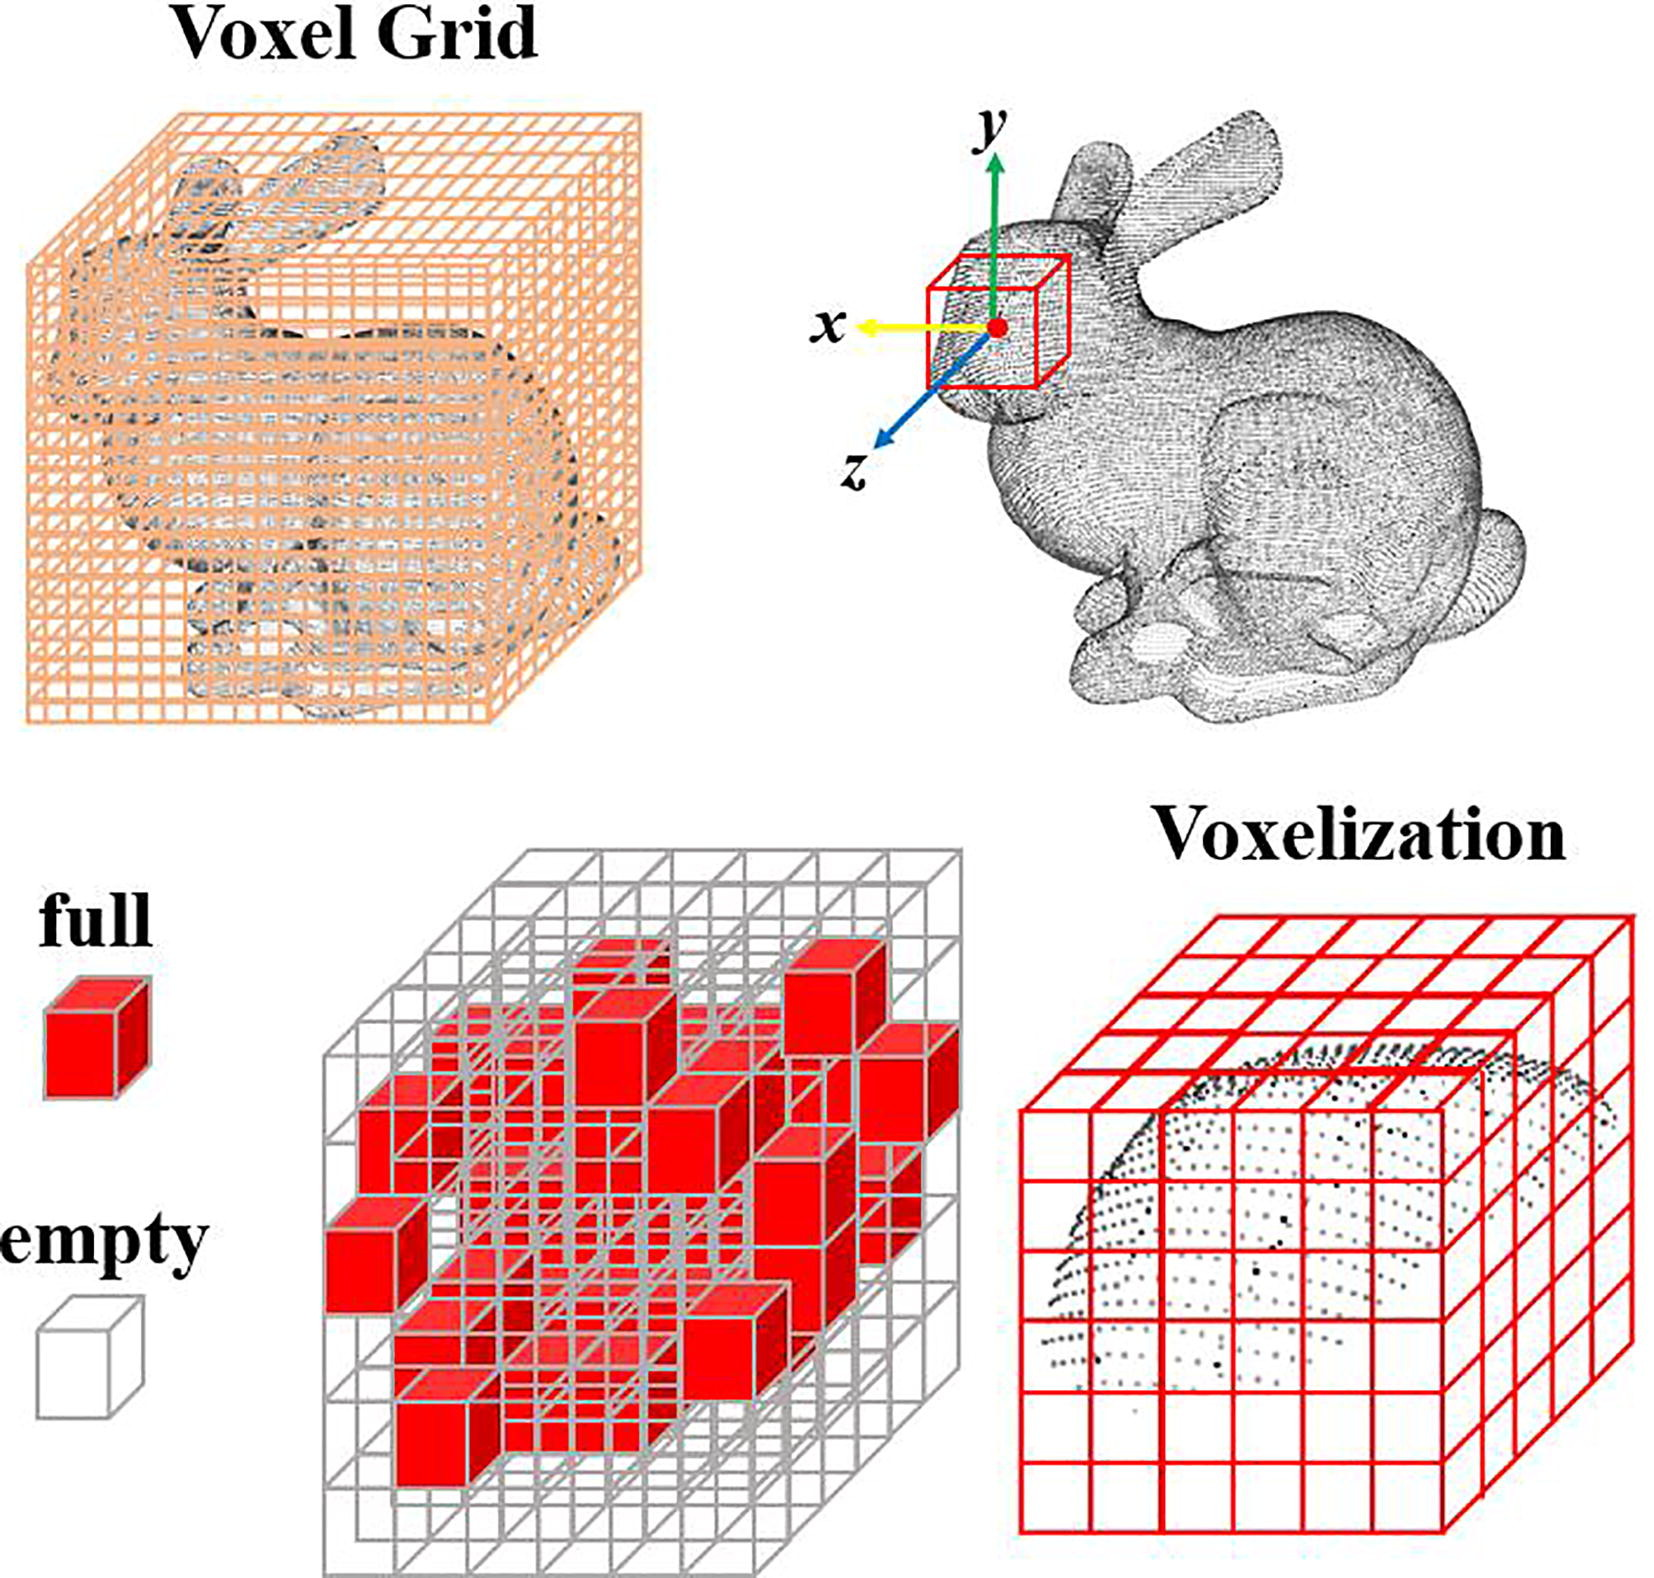
\includegraphics[width=\textwidth]{voxel}
        \end{columns}
    \end{frame}


    \begin{frame}{Limitations of Voxelization based compression}
        \begin{columns}
            \column{0.5\textwidth}
            \only<1>{
                \begin{itemize}
                \item Quantization error
                \item Larger representation volume
                \item Hard to train a single model for variable bitrates
                \end{itemize}
            }
            \vspace{20pt}
            \textbf{Solution:} Voxelization free compression
            \column{0.5\textwidth}
            \centering
            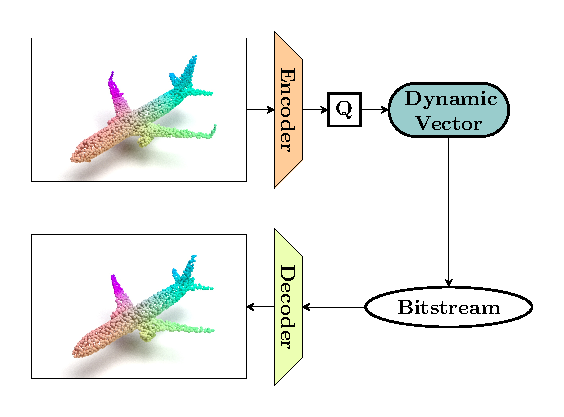
\includegraphics[width=\textwidth]{overview}
            \tiny Fig: Voxelization free compression pipeline
        \end{columns}
    \end{frame}


     \begin{frame}{Architecture Overview}
        \only<1>{
            \begin{itemize}
                \item Permutation invariant encoder
                \item Multiple Decoder branch
                \item Trained to minimize loss defined on unordered Sets
                %\item but only 2 million \textbf{axons} (optic nerve endings)
            \end{itemize}
            \vspace{20pt}
            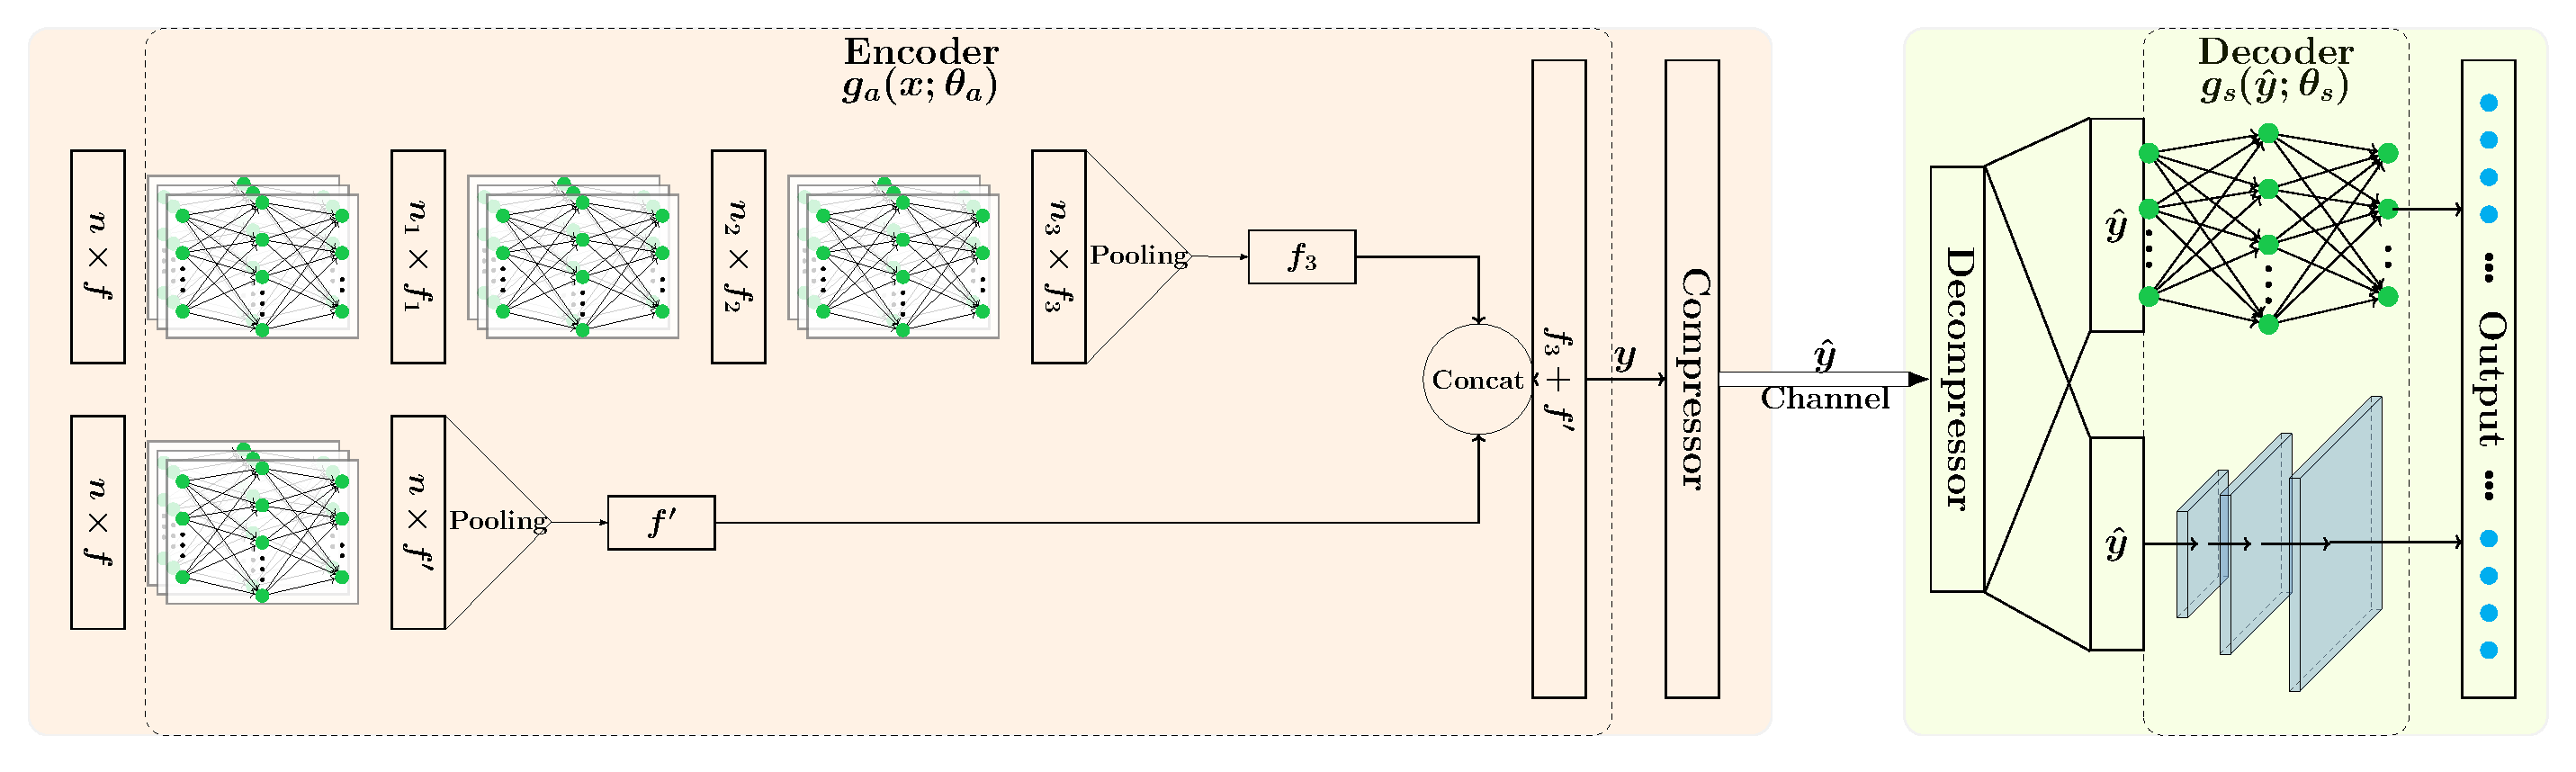
\includegraphics[width=\textwidth]{model_architecture}
        }
    \end{frame}


     \begin{frame}{Multi decoder}
        \begin{columns}
            \column{0.4\textwidth}
            \only<1>{
                \begin{itemize}
                \item Many objects, especially man-made objects, contain large smooth surfaces
                \item Deconvolution can generate locally smooth surface
                \item A fully-connected network combined with a deconvolutional network performs best
                \end{itemize}
            }
            \column{0.6\textwidth}
            \centering
            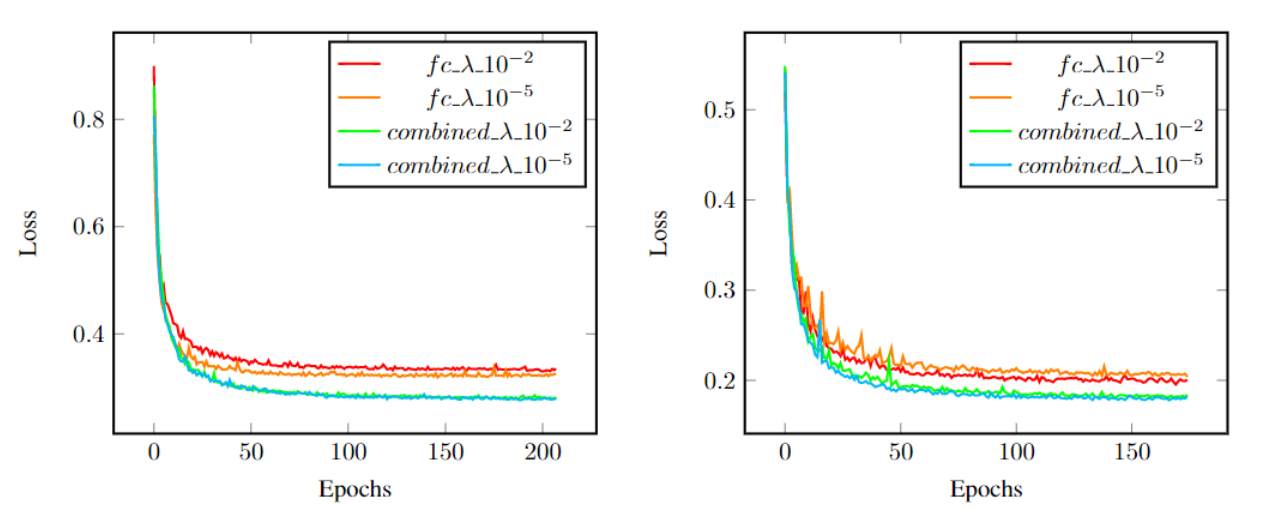
\includegraphics[width=\textwidth]{multidecoder}
            \tiny Fig: Performance on ModelNet40 (Left), Performance on ShapeNet (Right)
        \end{columns}
    \end{frame}


    \begin{frame}{Variable compression rate}
        \begin{columns}
            \column{0.5\textwidth}
            \only<1>{
                \begin{itemize}
                    \item Traditional Formulation
                        \[ L = D + \lambda R\]
                        \[ R = E_x[-\log P_{\hat{y}}(Q(g_a(x;\theta_a)))] \]

                    \item Weighted Formulation
                        \[ R_{weighted} = E_x[\sum_{i} -\omega_i \log P(\hat{y}_i)]\]
                       \[ \omega_i = a e^{-b\times i}\]
                \end{itemize}

            }
            \column{0.5\textwidth}
            %\centering
%            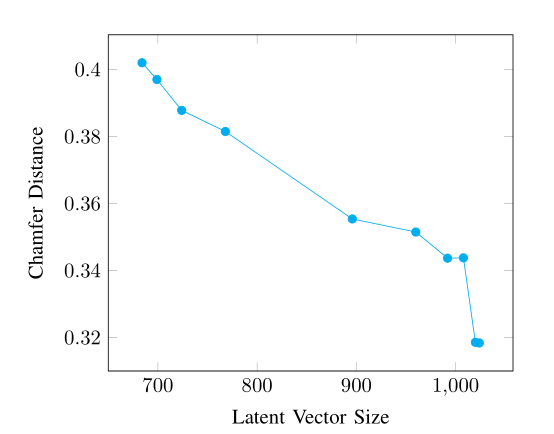
\includegraphics[width=\textwidth]{var_bitrate}
            \begin{figure}
                \centering
                \begin{tikzpicture}
                \begin{axis}[ xlabel=Latent Vector Size, ylabel=Chamfer Distance, width=\textwidth]%, x dir=reverse
                  \addplot[mark=*,cyan] plot coordinates {(1024,0.3184) (1020,0.3186)
                  (1024-16,0.3438) (1024-32,0.3437) (1024-64,0.3515) (1024-128,0.3554)
                  (1024-256,0.3815) (1024-300,0.3878) (1024-325,0.397) (1024-340,0.402)
                  %(1024-343,1.14) (1024-512,2.283)
                };
                %\addlegendentry{EMD}
                \end{axis}
                \end{tikzpicture}

                \end{figure}
        \end{columns}
    \end{frame}


    \begin{frame}{Experiment}
            \only<1>{
                \begin{itemize}
                    \item Dataset: ShapeNet, ModelNet40
                \end{itemize}
                \vspace{20pt}
                %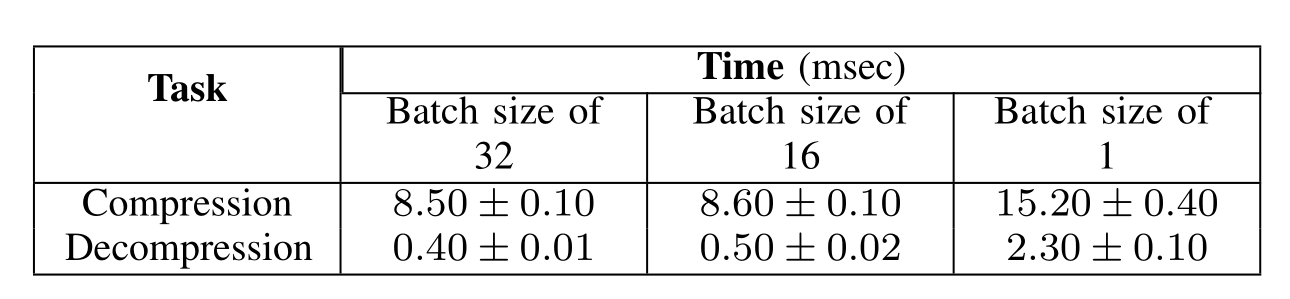
\includegraphics[width=\textwidth]{timing}
                \newcolumntype{C}{>{\centering\arraybackslash}p{0.2\linewidth}}
                \begin{table}
                \begin{center}
                \begin{tabular}{|C|C|C|C|} % <-- Alignments: 1st column left, 2nd middle and 3rd right, with vertical lines in between
                  \hline
                  \multirow{2}{*}{\textbf{Task}} & \multicolumn{3}{|c|}{\textbf{Time} (msec)}\\
                  \cline{2-4}&
                   Batch size of 32 & Batch size of 16 & Batch size of \newline 1\\
                    \hline
                    Compression   & $8.50 \pm0.10$ & $8.60 \pm0.10$ & $15.20 \pm0.40$\\
                    Decompression & $0.40 \pm0.01$ & $0.50 \pm0.02$ & $2.30 \pm0.10$\\
                  \hline
                \end{tabular}
                \end{center}
                \end{table}
            }
    \end{frame}


     \begin{frame}{Qualitative results}
            \only<1>{
                \vspace{0pt}
                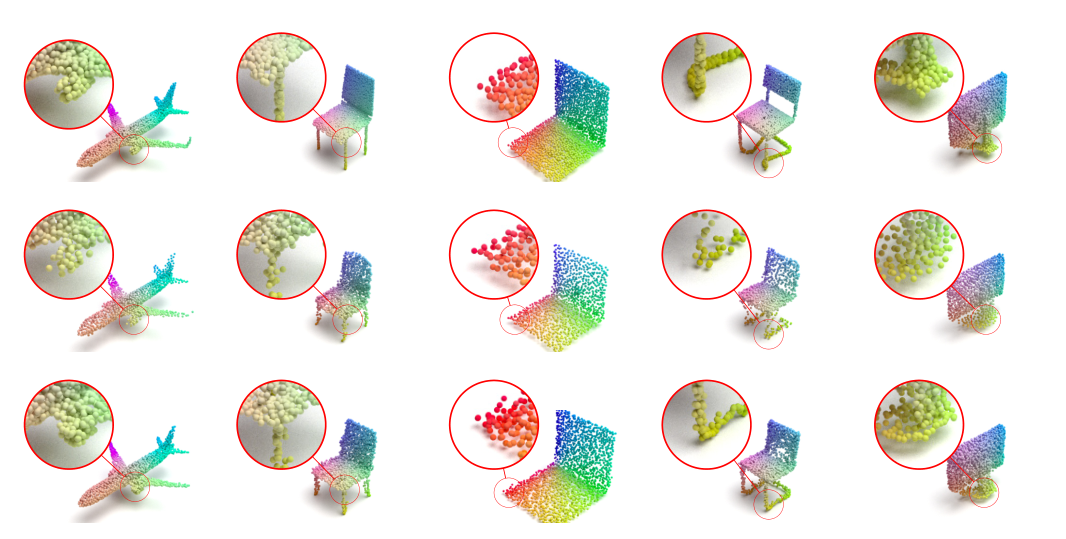
\includegraphics[width=.98\textwidth]{qualitative}
            }
    \end{frame}


    \begin{frame}{Quantitative results}
        \begin{columns}
            \column{0.5\textwidth}
            \only<1>{
                \begin{itemize}
                    \item Our method produces significantly better results at low bitrates compared to the
                    Draco
                \end{itemize}
            }
            \column{0.5\textwidth}
%            \centering
%            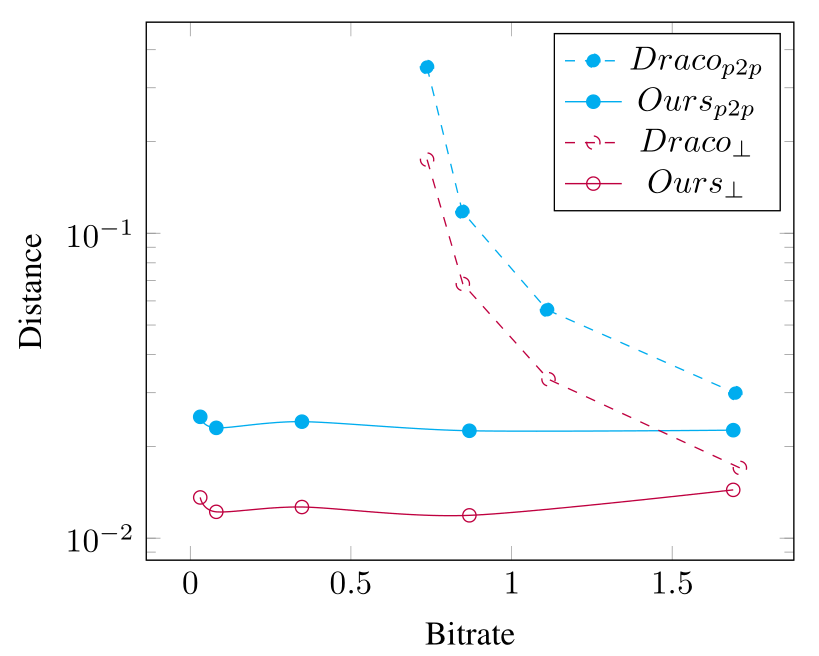
\includegraphics[width=\textwidth]{draco}
            \begin{figure}
                \centering
                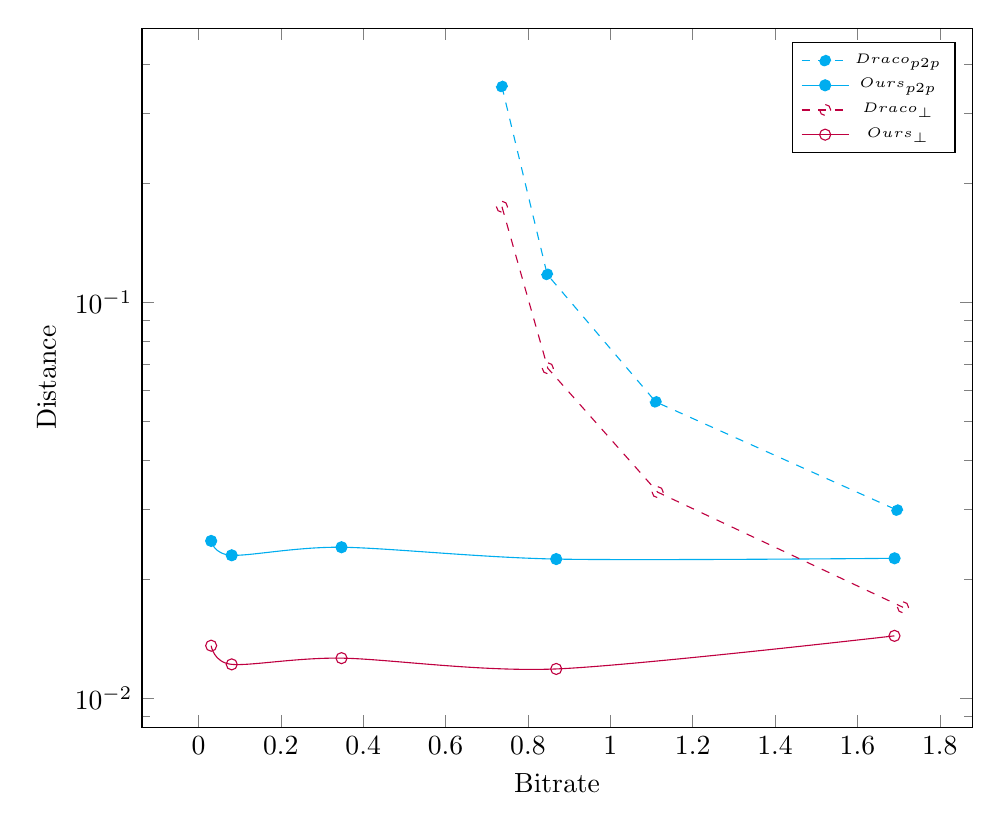
\begin{tikzpicture}
                  \begin{axis}[xlabel=Bitrate,ylabel=Distance,ymode=log,width=\textwidth,]
                    \addplot[dashed,mark=*,color=cyan] plot coordinates { (0.7368, 0.3509) (0.8468, 0.1177)(1.11034, 0.0561) (1.6965, 0.0299)};%(3.0663, 0.01909)
                    \addlegendentry{\tiny$Draco_{p2p}$}
                    \addplot[smooth,mark=*,color=cyan] plot coordinates { (0.0309,0.025) (0.0808, 0.023) (0.3474,0.0241 ) (0.8687,0.0225 )(1.690192, 0.0226) };
                    % 0.0212, 0.0186, 0.0199,0.0175, 0.01804
                    \addlegendentry{\tiny$Ours_{p2p}$}
                    \addplot[dashed,mark=o,color=purple] plot coordinates { (0.737, 0.1744) (0.8483, 0.0682) (1.115, 0.0332) (1.7107, 0.0170)}; %(3.1040, 0.0105)
                    \addlegendentry{\tiny$Draco_\perp$}
                    \addplot[smooth,mark=o,color=purple] plot coordinates { (0.0309, 0.0136) (0.0808,  0.0122) (0.3474, 0.01265 ) (0.8687, 0.01188)(1.690, 0.0144 ) };
                    %0.0112, 0.0096, 0.0103,  0.0092, 0.0095
                    \addlegendentry{\tiny$Ours_\perp$}
                  \end{axis}
                \end{tikzpicture}
                \label{fig:draco_comparison}
                \end{figure}
        \end{columns}
    \end{frame}


    \begin{frame}{Quantitative results}
        \begin{columns}
            \column{0.5\textwidth}
            \only<1>{
                \begin{itemize}
                    \item Decompressed point cloud retains the semantic structure
                \end{itemize}
            }
            \column{0.5\textwidth}
%            \centering
%            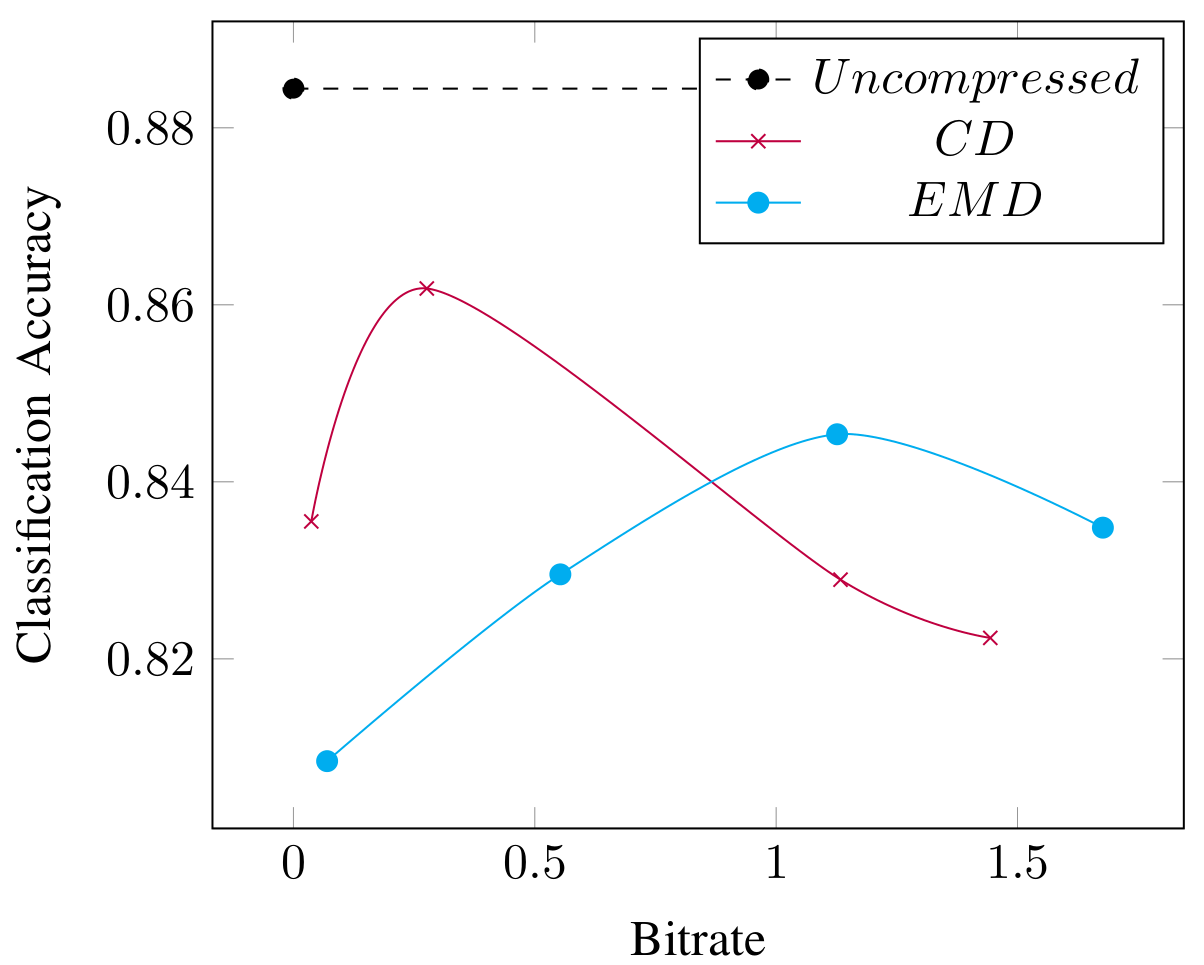
\includegraphics[width=\textwidth]{cls_accuracy}
            \begin{figure}
                \centering
                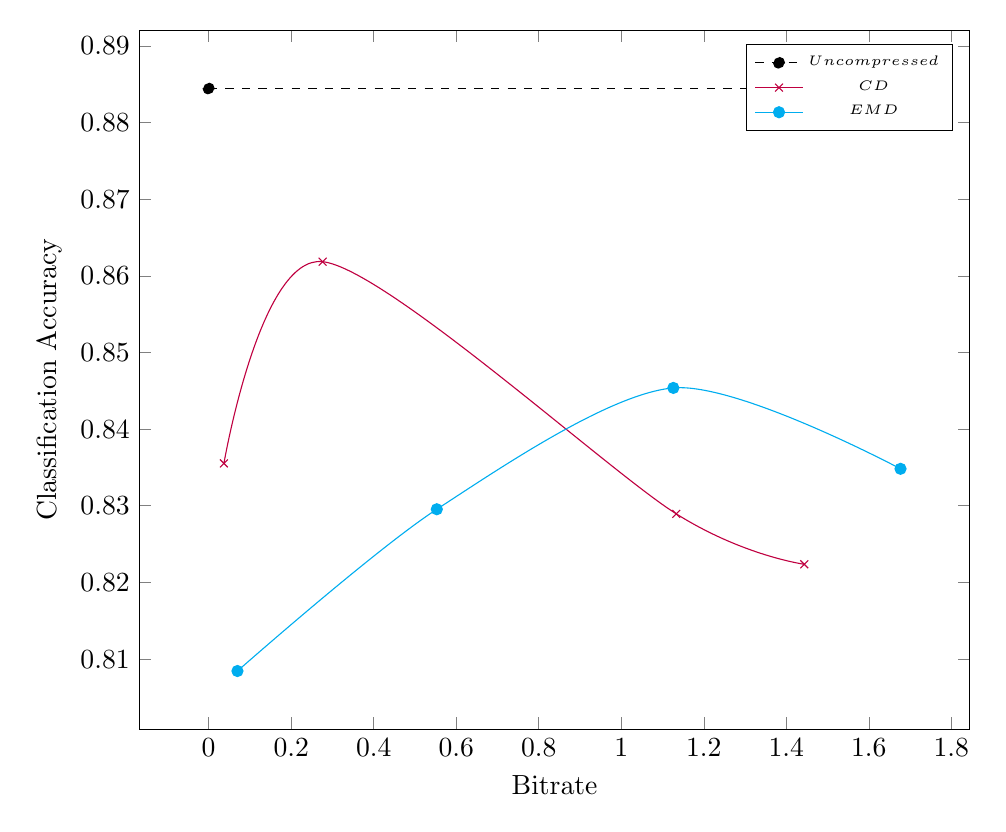
\begin{tikzpicture}
                  \begin{axis}[xlabel=Bitrate,ylabel=Classification Accuracy, width=\textwidth]
                  \addplot[dashed,mark=*,color=black] plot coordinates { (0.0, 0.88442) (1.676785, 0.88442) };
                  \addlegendentry{\tiny$Uncompressed$}
                  \addplot[smooth,mark=x,color=purple] plot coordinates { (0.036987, 0.835526) (0.276215, 0.861842) (1.133270, 0.828947) (1.443545, 0.822368) };
                  \addlegendentry{\tiny$CD$}
                  \addplot[smooth,mark=*,color=cyan] plot coordinates { (0.069773, 0.808442) (0.552924, 0.829545) (1.126253, 0.845373) (1.676785, 0.834821) };
                  \addlegendentry{\tiny$EMD$}
                  \end{axis}
                \end{tikzpicture}
                \end{figure}
        \end{columns}
    \end{frame}


% % -------------------------------------------------------------------------------------------------
% % extro
% % -------------------------------------------------------------------------------------------------
\begin{frame}{}
\centering
{\Huge \calligra Thank you}
%Thank you
\end{frame}

\end{document}

